\section{ Vorausberechnung der Schaltung}

Zur Vorbereitung werden die Grundverstärkungen und Grenzfrequenzen von Hoch- und Tiefpass, die Mittenfrequenz und Bandbreite des Bandpasses und die Sperrfrequenz der Bandsperre berechnet.

\subsection{Grundverstärkung und Grenzfrequenzen der Hoch- und Tiefpässe}
Aus Anlage 7 Lassen sich die folgenden Formeln für Hoch und Tiefpässe entnehmen:

% grafik einbinden
\begin{figure}[H]
    \begin{center}
        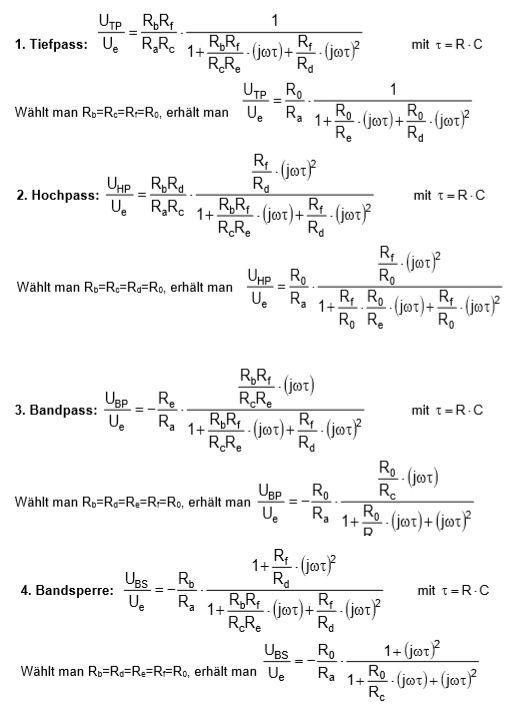
\includegraphics[width=0.8\textwidth]{img/grundamp.png}
        \caption{Frequenzgänge aus Anlage 7 von "GNP3 Aktive RC-Filter.pdf"} %Vorlesung GN Kapitel 5 Filter, Seite 43}
        \label{fig:V1_filter}
    \end{center}
\end{figure}



\iffalse%%%%%%%%%%%%%%%%%%%%%%%%%%%%%%%%%%%%%%%%%%%%%%%%%%%%%%%%%%%%%%%%%%%%%%%%%%%
Die Grenzfrequenz für Hoch- und Tiefpässe lässt sich über die folgende Formel bestimmen:

\[ f_g = \frac{1}{2\pi R C} = \frac{1}{2\pi \cdot \SI{10}{\kilo\ohm} \cdot \SI{10}{\nano\farad}} = \SI{1591,5}{\hertz} \]


Die Grundverstärkung wird für die Tiefpässe über die folgende Formel berechnet:
\[ v_0 = \frac{R_B R_F}{R_A R_C} = \frac{\SI{3.32}{\kilo\ohm} \cdot \SI{3.32}{\kilo\ohm}}{\SI{3.32}{\kilo\ohm} \cdot \SI{3.32}{\kilo\ohm}} = 1 \]


Für die Hochpässe wird diese Formel verwendet:

\[ v_\infty = \frac{R_B R_D}{R_A R_C} = \frac{\SI{3.32}{\kilo\ohm} \cdot  \SI{3.32}{\kilo\ohm}}{\SI{3.32}{\kilo\ohm} \cdot \SI{3.32}{\kilo\ohm}} = 1 \]


\fi%%%%%%%%%%%%%%%%%%%%%%%%%%%%%%%%%%%%%%%%%%%%%%%%%%%%%%%%%%%%%%%%%%%%%%%%%%%%%%%

\subsection{Mittenfrequenz und Bandbreite des Bandpasses }

Die Mittenfrequenz wird mit der folgenden Formel berechnet:

\[ f_0 = \frac{1}{2\pi R C} = \frac{1}{2\pi \cdot \SI{10}{\kilo\ohm} \cdot \SI{10}{\nano\farad}} = \SI{1591,5}{\hertz} \]




\newpage

Die Bandbreite wird mit der folgenden Formel berechnet:

\[ b = \frac{R_B R_F}{R_C R_E} \cdot f_0 = \frac{\SI{3.32}{\kilo\ohm} \cdot  \SI{3.32}{\kilo\ohm}}{\SI{16,5}{\kilo\ohm} \cdot \SI{3.32}{\kilo\ohm}} \cdot \SI{1591,5}{\hertz} = \SI{320,23}{\hertz} \]


\subsection{Sperrfrequenz der Bandsperre }

Die Sperrfrequenz wird mit der folgenden Formel berechnet:

\[ f_0 = \frac{1}{2\pi R C} = \frac{1}{2\pi \cdot \SI{10}{\kilo\ohm} \cdot \SI{10}{\nano\farad}} = \SI{1591,5}{\hertz} \]

\subsection{Übertragungsfunktionen mit Matlab symbolisch berechnet}

% TODO

\subsection{Übertragungsfunktionen (Betrag und Phase) mit Matlab numerisch berechnet}

Die Übertragungsfunktionen der verschiedenen Filter werden in Matlab numerisch berechnet und geplottet. In \autoref{fig:A2_tiefpaesse} sind die Tiefpässe dargestellt. In \autoref{fig:A2_hochpaesse} sind die Hochpässe dargestellt. In \autoref{fig:A2_band} sind der Bandpass und die Bandsperre dargestellt.

\begin{figure}[H]
    \begin{center}
        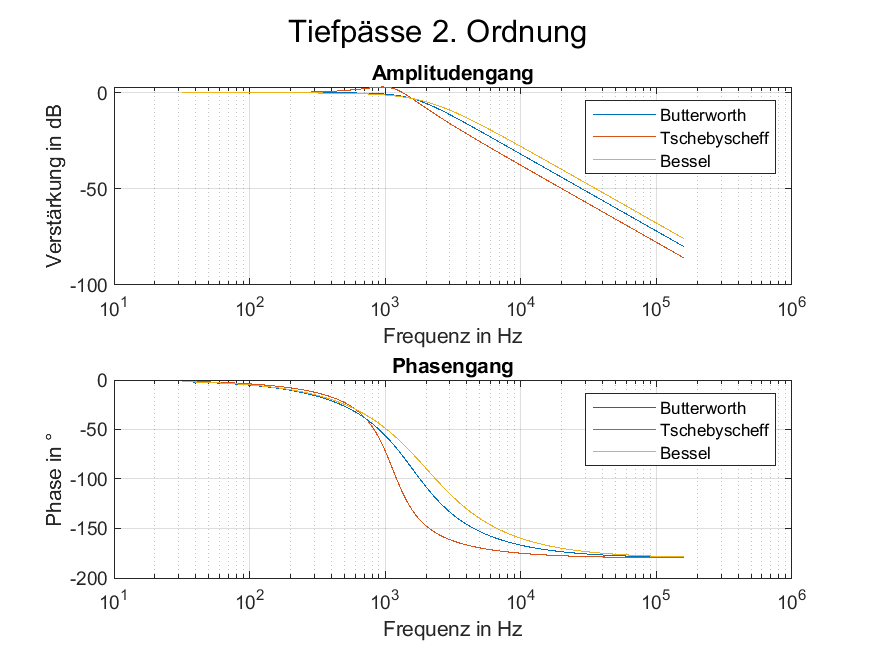
\includegraphics[width=0.8\textwidth]{img/Aufgabe2_5_Tiefpaesse.png}
        \caption{Numerisch berechneter Bodeplot der verschiedenen Tiefpässe}
        \label{fig:A2_tiefpaesse}
    \end{center}
\end{figure}

\begin{figure}[H]
    \begin{center}
        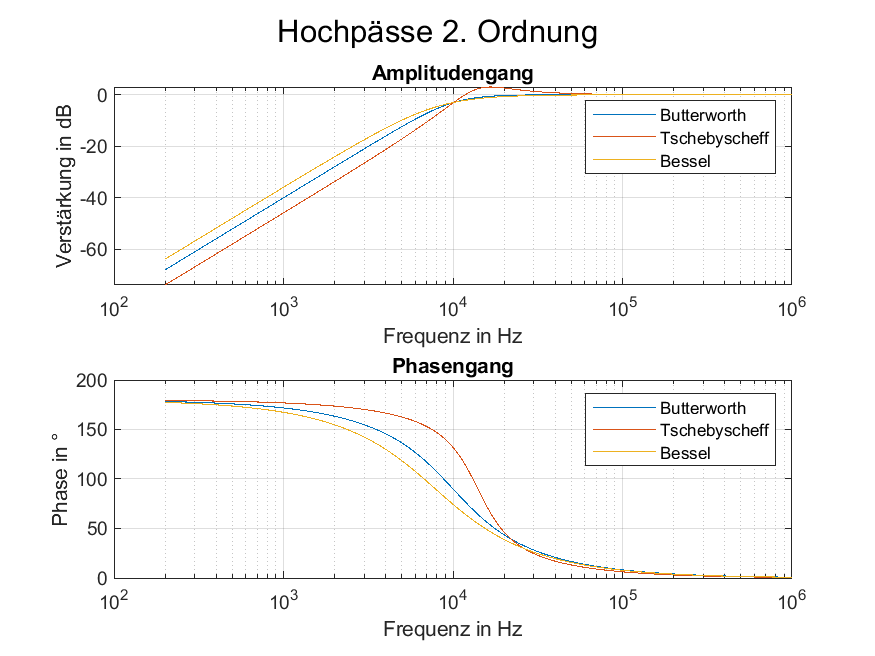
\includegraphics[width=0.8\textwidth]{img/Aufgabe2_5_Hochpaesse.png}
        \caption{Numerisch berechneter Bodeplot der verschiedenen Hochpässe}
        \label{fig:A2_hochpaesse}
    \end{center}
\end{figure}

\begin{figure}[H]
    \begin{center}
        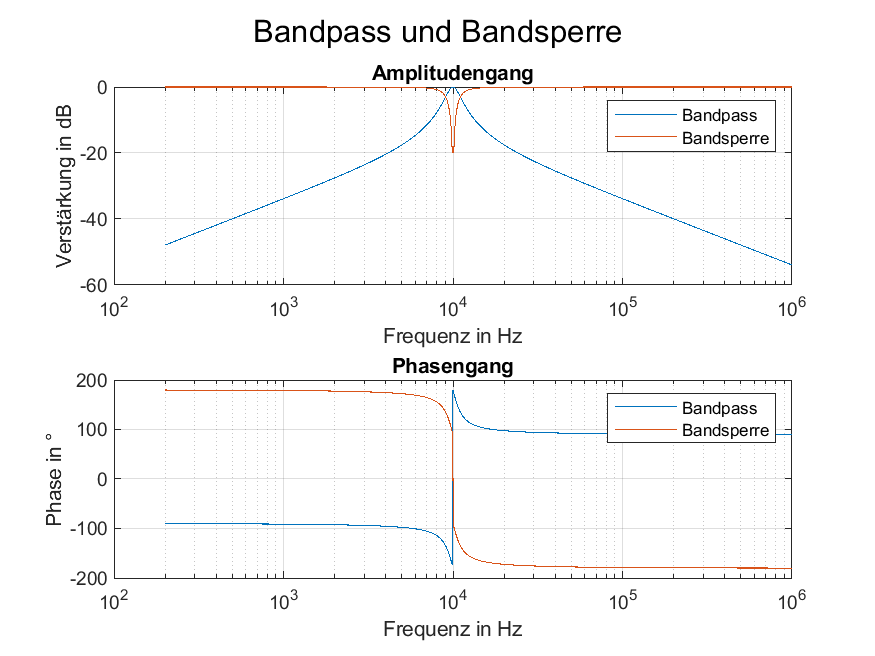
\includegraphics[width=0.8\textwidth]{img/Aufgabe2_5_Band.png}
        \caption{Numerisch berechneter Bodeplot von Bandpass und -sperre}
        \label{fig:A2_band}
    \end{center}
\end{figure}

\subsection{Spice Simulationsergebnisse für das Frequenzverhalten (AC-Analyse)}

%Die Eigenschaften 1-3) können entweder berechnet (siehe Abschnitte 6 und 7) oder aus Simulationen mit Spice (z.B. PSpice oder LTSpice) entnommen werden. Der Berechnungsgang bzw. Schaltung und Plot der Spice-Simulation sind zum Labortermin vorzulegen und in das Protokoll mit aufzunehmen, genauso wie der Matlab-Code.

% grafik einbinden
\begin{figure}[H]
    \begin{center}
        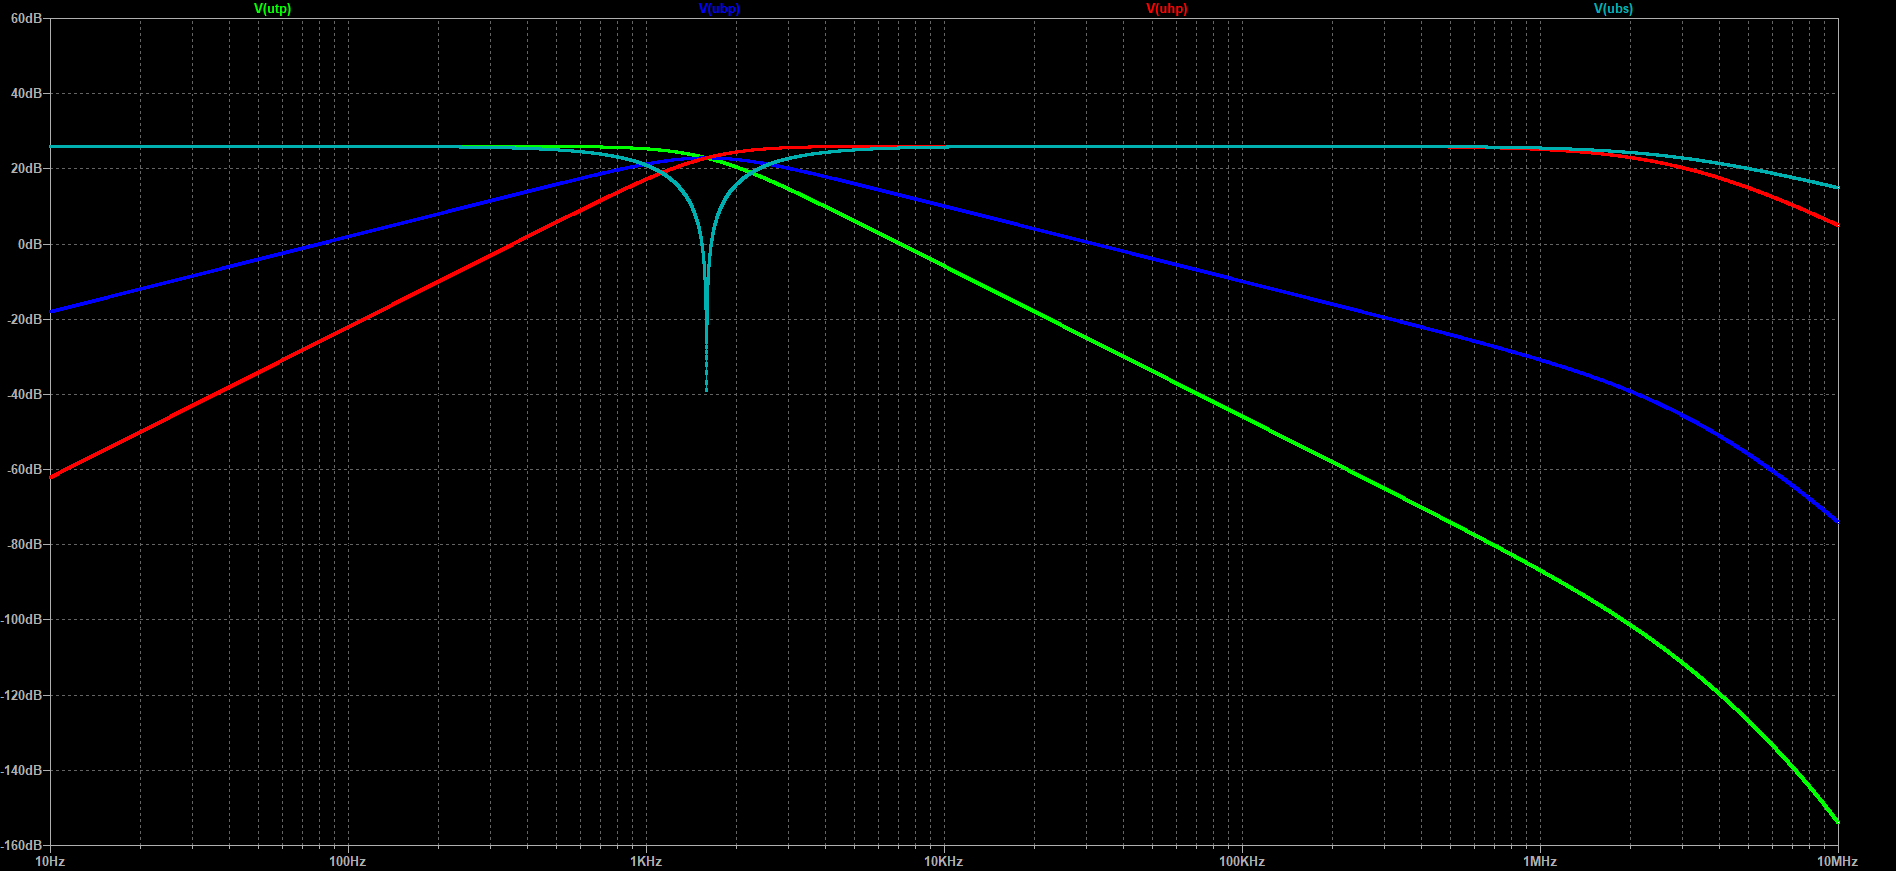
\includegraphics[width=1\textwidth]{img/LTsim.png}
        \caption{Simulation der Schaltung in LTspice }
        \label{fig:V4_Sim}
    \end{center}
\end{figure}
\begin{figure}[H]
    \begin{center}
        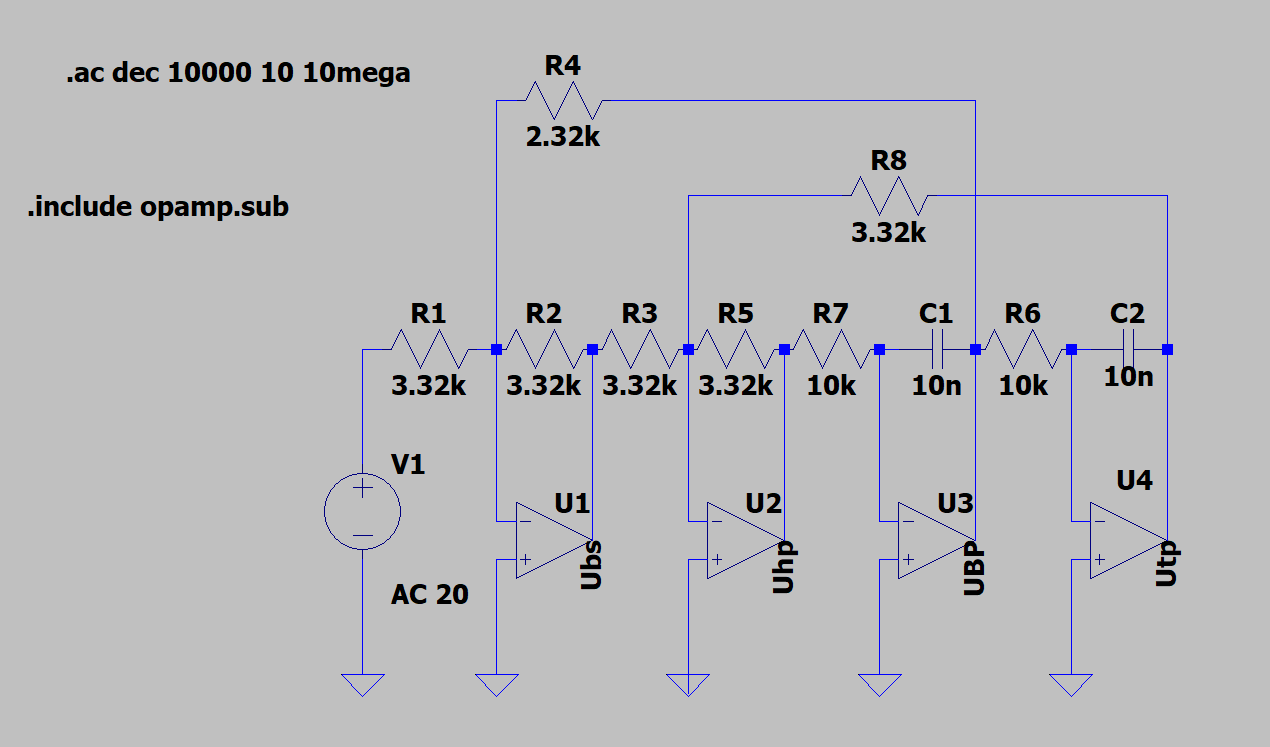
\includegraphics[width=0.5\textwidth]{img/LTblock.PNG}
        \caption{Schaltung in LTspice}
        \label{fig:V4_Block}
    \end{center}
\end{figure}

Zu erkennen ist die Grenzfrequenz der Filter bei $f_g= \SI{1591.5}{\hertz}$.



